\documentclass[10pt]{report}

\usepackage{geometry}
\geometry{
	a4paper,
	margin=1in,
	footskip=0.25in
}

\usepackage{enumerate} % for enumerate counter
\usepackage{subcaption} % for subfigures
\usepackage{amsthm} % for QED
\usepackage{mathtools} % for delimiter

\usepackage{listings} % for code
\lstset{ 
	language=R,
	basicstyle=\footnotesize\ttfamily,
	numbers=none,
	stepnumber=1,
	numbersep=8pt,
	showspaces=false,
	showstringspaces=false,
	showtabs=false,
	frame=single,
	tabsize=2,
	captionpos=t,
	breaklines=true,
	breakatwhitespace=false
} 

\usepackage{float} % for figure [H]
\usepackage{booktabs} % for tabular
\usepackage{caption} % for \caption*
\usepackage[export]{adjustbox} % for valign=t
\usepackage{array} % for column type m
\usepackage{verbatim}
\usepackage{graphicx}
%\graphicspath{ {imgs/} }

\usepackage{fancyhdr}
\pagestyle{fancy}
\fancyhead[L]{\hwAuther}
\fancyhead[C]{\courseNo}
\fancyhead[R]{\hwNo}

\usepackage{amssymb}
\usepackage{amsmath}

%Cover
\newcommand{\courseTitle}{Introduction to Mathematical Modeling}
\newcommand{\courseNo}{Math 380}
\newcommand{\hwAuther}{Zhihao Ai}

\newcommand{\hwNo}{HW \#2}
\newcommand{\hwDate}{Due on 02/06}

\title{
	\courseTitle\\
	\hwNo\\
	\hwDate
}
\author{\hwAuther}
\date{}
%

%Custom
%\everymath{\displaystyle}
\setlength\parindent{0pt}

%Custom commands
\newcommand{\ds}{\displaystyle}
\newcommand{\ts}{\textstyle}

\newcolumntype{N}{>$ c <$} 
\newcolumntype{M}[1]{>{\centering\arraybackslash $}m{#1}<{$}}

\newcommand{\abs}[1] {\left| #1 \right|}

\DeclarePairedDelimiter\autoparen{(}{)}
\newcommand{\pa}[1]{\autoparen*{#1}}

\newcommand{\var} {\text{var}}

\newcommand{\m}[1] {\mathbf{#1}}

\begin{document}

\maketitle



\section*{Section 1.3}
\begin{enumerate}
	\item [1f.]
	Find the solution to the difference equation:
	\[a_{n+1} = 0.1 a_n + 3.2, \quad a_0 = 1.3\]
	Since $r \ne 1$, from Theorem 3, we have
	\[
	a_n = r^n c + \frac{b}{1-r} = (0.1)^n c + \frac{3.2}{0.9}
	\]
	Let $n = 0$,
	\[
	a_0 = (0.1)^0 c + \frac{32}{9} = 1.3 \to c = - \frac{203}{90}
	\]
	Therefore, the solution is
	\[
	a_n = -(0.1)^n \frac{203}{90} + \frac{32}{09}
	\]
	
	\item [2e.]
	Find an equilibrium value if one exists. Classify the equilibrium values as stable or unstable.
	\[a_{n+1} = -1.2 a_n + 50\]
	From Theorem 2, the equilibrium value is
	\[
	a = \frac{b}{1-r} = \frac{50}{-1.2} = \frac{250}{11}
	\]
	Since $\abs{r} = 1.2 > 1$, it is an unstable equilibrium.
	
	\item [3a.]
	Build a numerical solution for the following \textit{initial value problem}. Plot your data to observe patterns in the solution. Is there an equilibrium solution? Is it stable or unstable?
	\[a_{n+1} = -1.2 a_n + 50, \quad a_0 = 1000\]
	Since $r \ne 1$, from Theorem 3 and problem 2e, we have
	\[
	a_n = r^n c + \frac{b}{1-r} = (-1.2)^n c + \frac{250}{11}
	\]
	Let $n = 0$,
	\[
	a_0 = (-1.2)^0 c + \frac{250}{11} = 1000 \to c = \frac{10750}{11}
	\]
	Therefore, the solution is
	\[
	a_n = (-1.2)^n \frac{10750}{11} + \frac{250}{11}
	\]
	\begin{figure}[H]
		\centering
		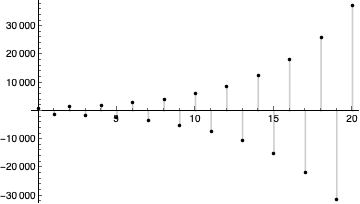
\includegraphics[width=0.5\linewidth]{s1_3/3a.png}
	\end{figure}
	There is no equilibrium solution.
	
	\item [6.]
	You owe \$500 on a credit card that charges 1.5\% interest each month. You can pay \$50 each month with no new charges. What is the equilibrium value? What does the equilibrium value mean in terms of the credit card? Build a numerical solution. When will the account be paid off? How much is the last payment?
	
	Denote the amount on the credit card after $n$ months as $a_n$. We have
	\begin{align*}
		a_{n+1} &= 1.015 a_n - 50, \quad n=0,1,2,3,\dots\\
		a_0 &= 500
	\end{align*}
	From Theorem 2, the equilibrium value is
	\[
	a = \frac{b}{1-r} = \frac{-50}{1-1.015} = 3333.33
	\]
	meaning that if the amount on credit card is \$3333.33, it would stay the same for every month afterwards. From Theorem 3, the solution to the system is
	\[
	a_n = r^n c + \frac{b}{1-r} = (1.015)^n c + \frac{-50}{-0.015}
	\]
	Let $n = 0$,
	\[
	a_0 = (1.015)^0 c + \frac{10000}{3} = 500 \to c = -\frac{8500}{3}
	\]
	When the account is paid off ($a_n = 0$), $n$ is about 10.9157, meaning it would be paid off after 11 months. The last payment is what's left after 10 months, which is $a_{10} = -(1.015)^{10} \frac{8500}{3} + \frac{10000}{3} = 45.13$.
	
	\item [10.]
	Find the equilibrium value of the digoxin model. What is the significance of the equilibrium value? (Instead of Example 4, Section 1.2, use $a_{n+1} = 0.69 a_n + 0.1, a_0=0.5$)
	
	From Theorem 2, the equilibrium value is
	\[
	a = \frac{b}{1-r} = \frac{0.1}{1-0.69} = 0.323
	\]
	Since $\abs{r} < 1$, the equilibrium value is stable, meaning that no matter how much the inital dose is, at a daily dosage of 0.1mg, the concentration level will approach 0.323 and stay the same afterwards.
\end{enumerate}

\section*{Section 1.4}
\begin{enumerate}
	\item [2.]
	Consider Example 3, Competitive Hunter Model--Spotted Owls and Hawks. Experiment with different values for the coefficients using the starting values given. Then try different starting values. What is the long-term behavior? Do your experimental results indicate that the model is sensitive
	\begin{enumerate}[a.]
		\item 
		to the coefficients?
		\begin{figure}[H]
			\centering
			\begin{subfigure}[b]{.5\linewidth}
				\caption{$k_1 = 0.19, k_2 = 0.31, k_3 = 0.001, k_4 = 0.002$}
				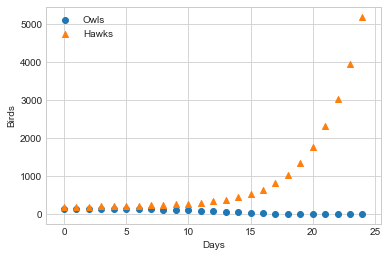
\includegraphics[width=\linewidth]{s1_4/k12-1.png}
			\end{subfigure}%%
			\begin{subfigure}[b]{.5\linewidth}
				\caption{$k_1 = 0.21, k_2 = 0.29, k_3 = 0.001, k_4 = 0.002$}
				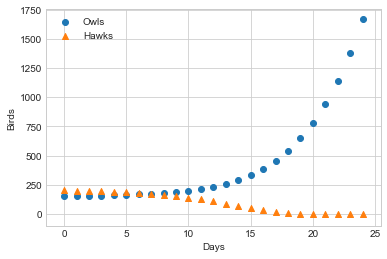
\includegraphics[width=\linewidth]{s1_4/k12-2.png}
			\end{subfigure}
		\end{figure}
		\begin{figure}[H]\ContinuedFloat
			\begin{subfigure}[b]{.5\linewidth}
				\caption{$k_1 = 0.2, k_2 = 0.3, k_3 = 0.0009, k_4 = 0.0021$}
				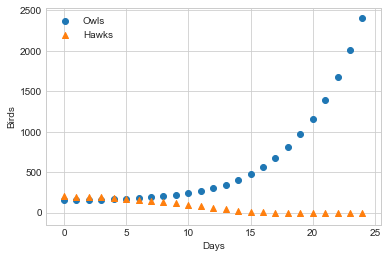
\includegraphics[width=\linewidth]{s1_4/k34-1.png}
			\end{subfigure}%%
			\begin{subfigure}[b]{.5\linewidth}
				\caption{$k_1 = 0.2, k_2 = 0.3, k_3 = 0.0011, k_4 = 0.0019$}
				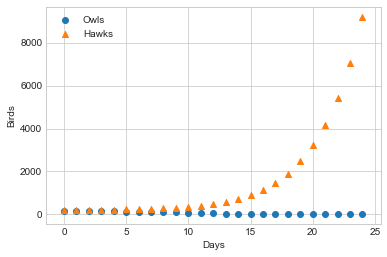
\includegraphics[width=\linewidth]{s1_4/k34-2.png}
			\end{subfigure}
		\end{figure}
		In plot (a) and (d) hawks drive owls to extinction. In plot (b) and (c) owls drive hawks to extinction. The results indicate the model is sensitive to the coefficients.
		
		\item 
		to the starting values?
		\begin{figure}[H]
			\centering
			\begin{subfigure}[b]{.3\linewidth}
				\caption{$O_0 = 149, H_0 = 201$}
				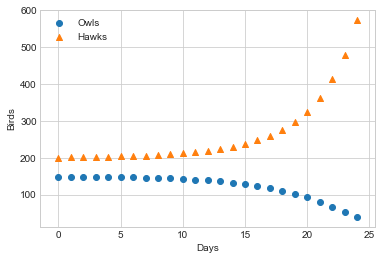
\includegraphics[width=\linewidth]{s1_4/oh-1.png}
			\end{subfigure}
			\begin{subfigure}[b]{.3\linewidth}
				\caption{$O_0 = 151, H_0 = 199$}
				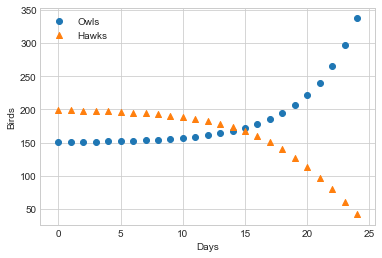
\includegraphics[width=\linewidth]{s1_4/oh-2.png}
			\end{subfigure}
			\begin{subfigure}[b]{.3\linewidth}
				\caption{$O_0 = 10, H_0 = 10$}
				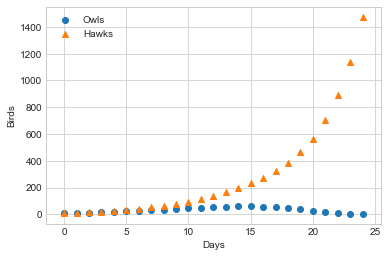
\includegraphics[width=\linewidth]{s1_4/oh-3.png}
			\end{subfigure}
		\end{figure}
	\end{enumerate}
	In plot (a) and (c) hawks drive owls to extinction. In plot (b) owls drive hawks to extinction. The results indicate the model is sensitive to the starting values.

	\item [4.]
	Suppose the spotted owls' primary food source is a single prey: mice. An ecologist wishes to predict the population levels of spotted owls and mice in a wildlife sanctuary. Letting $M_n$ represent the mouse population after $n$ years and $O_n$ the predator owl population, the ecologist has suggested the model
	\begin{align*}
		M_{n+1} &= 1.2 M_n - 0.001 O_n M_n\\
		O_{n+1} &= 0.7 O_n + 0.002 O_n M_n
	\end{align*}
	The ecologist wants to know whether the two species can coexist in the habitat and whether the outcome is sensitive to the starting populations.
	\begin{enumerate}[a.]
		\item 
		Compare the signs of the coefficients of the preceding model with the signs of the coefficients of the owls--hawks model in Example 3. Explain the sign of each of the four coefficients 1.2, -0.001, 0.7 and 0.002 in terms of the predator--prey relationship being modeled.
		
		1.2 means mouse population will increase by 20\% each year if there is no owl.\\
		-0.001 means owls preying on mice will decrease the mouse population.\\
		0.7 means owl population will decrease by 30\% each year if there is no mouse.\\
		0.002 means owls preying on mice will increase the owl population.
		
		\item 
		Test the initial populations in the following table and predict the long-term outcome:
		\begin{table}[H]
			\centering
			\begin{tabular}{*{3}{c}} 
				\toprule
				 & Owls & Mice\\ \midrule
				Case A & 150 & 200 \\
				Case B & 150 & 300 \\
				Case C & 100 & 200 \\
				Case D & 10 & 20 \\
				\bottomrule
			\end{tabular}
		\end{table}
		\begin{figure}[H]
			\centering
			\begin{subfigure}[b]{.5\linewidth}
				\caption{Case A}
				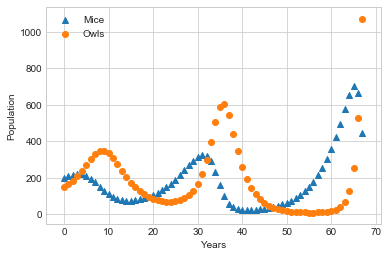
\includegraphics[width=\linewidth]{s1_4/caseA.png}
			\end{subfigure}%%
			\begin{subfigure}[b]{.5\linewidth}
				\caption{Case B}
				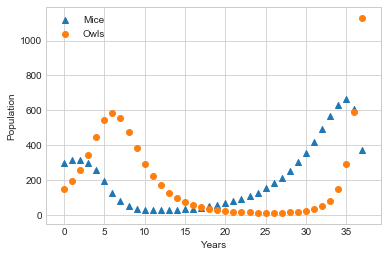
\includegraphics[width=\linewidth]{s1_4/caseB.png}
			\end{subfigure}
			\begin{subfigure}[b]{.5\linewidth}
				\caption{Case C}
				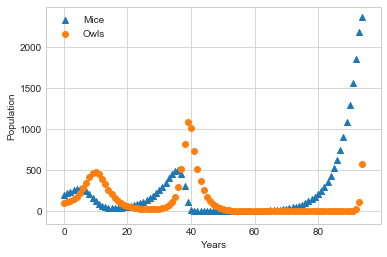
\includegraphics[width=\linewidth]{s1_4/caseC.png}
			\end{subfigure}%%
			\begin{subfigure}[b]{.5\linewidth}
				\caption{Case D}
				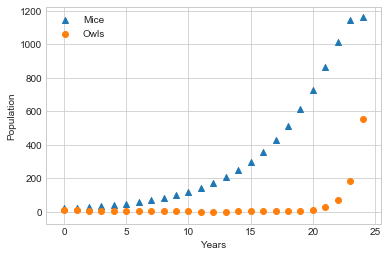
\includegraphics[width=\linewidth]{s1_4/caseD.png}
			\end{subfigure}
		\end{figure}
		The increase in mouse population will also cause increase in owl population. But more owls will reduce mouse population and as mouse population goes down, owls population will also go down. This pattern would go over and over again until at some time the product of owls and mice is so large that the growth of mice population is less than $0.001 O_n M_n$, leading to the extinction of mice.
		
		\item 
		Now experiment with different values for the coefficients using the starting values given. Then try different starting values. What is the long-term behavior? Do your experimental results indicate that the model is sensitive to the coefficients? Is it sensitive to the starting values?
		
		\begin{figure}[H]
			\centering
			\begin{subfigure}[b]{.5\linewidth}
				\caption{$1.2 \to 1.21, 0.7 \to 0.69$}
				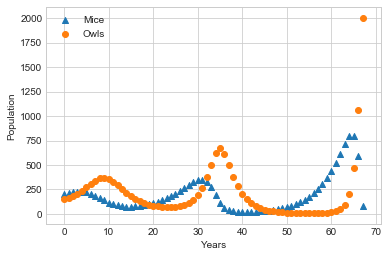
\includegraphics[width=\linewidth]{s1_4/4c1.png}
			\end{subfigure}%%
			\begin{subfigure}[b]{.5\linewidth}
				\caption{$0.001 \to 0.0011, 0.002 \to 0.0021$}
				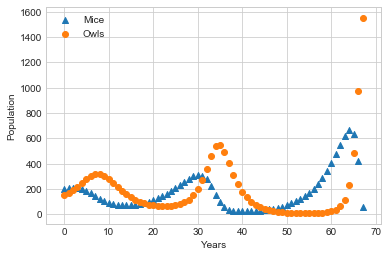
\includegraphics[width=\linewidth]{s1_4/4c2.png}
			\end{subfigure}
		\end{figure}
		\begin{figure}[H]\ContinuedFloat
			\begin{subfigure}[b]{.5\linewidth}
				\caption{$150 \to 149, 200 \to 201$}
				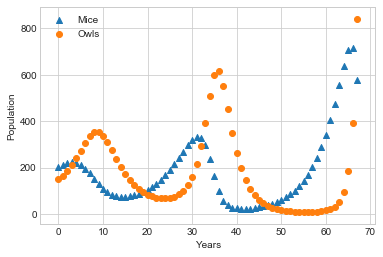
\includegraphics[width=\linewidth]{s1_4/4c3.png}
			\end{subfigure}%%
			\begin{subfigure}[b]{.5\linewidth}
				\caption{$150 \to 151, 200 \to 199$}
				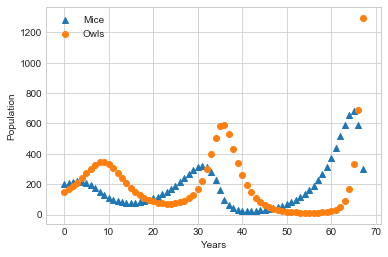
\includegraphics[width=\linewidth]{s1_4/4c4.png}
			\end{subfigure}
		\end{figure}
	\end{enumerate}
	The long-term behavior is owl driving mouse to extinction. The results indicate the model is relatively insensitive to both coefficients and starting values.
	
	%[Also try but do not submit #3]
\end{enumerate}

\section*{Section 2.2}
\begin{enumerate}
	\item [6.]
	Determine whether the following data support a proportionality argument for $y\propto z^{1/2}$. If so, estimate the slope.
	\begin{table}[H]
		\centering
		\begin{tabular}{*{6}{N}} 
			\toprule
			y & 3.5 & 5 & 6 & 7 & 8 \\ \midrule
			z & 3 & 6 & 9 & 12 & 15 \\
			\bottomrule
		\end{tabular}
	\end{table}
	Plotting $y$ against $z^{1/2}$, we have
	\begin{figure}[H]
		\centering
		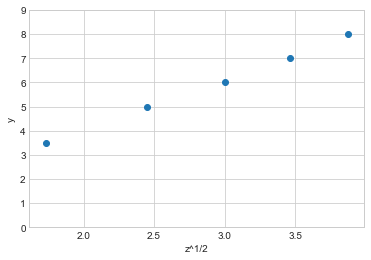
\includegraphics[width=0.5\linewidth]{s2_2/4.png}
	\end{figure}
	It's not a proportionality since the line does not pass through the origin.
\end{enumerate}

\section*{Section 2.3}
\begin{enumerate}
	\item [4.]
	Assume that under certain conditions the heat loss of an object is proportional to the exposed surface area. Relate the heat loss of a cubic object with side length 6 in. to one with a side length of 12 in. Now, consider two irregularly shaped objects, such as two submarines. Relate the heat loss of a 70-ft submarine to that of a 7-ft scale model. Suppose you are interested in the amount of energy needed to maintain a constant internal temperature in the submarine. Relate the energy needed in the actual submarine to that required by the scaled model. Specify the assumptions you have made.
	
	Since the exposed surface area $S$ of a cubic object is proportional to the square of its side length $l$, we have $S \propto l^2$. Because we assume the heat loss $L$ is proportional to the exposed surface area $S$, the relation between the heat loss of cubic object $CLoss_1$ with side length of 12 in. and of cubic object $CLoss_2$ with side length of 6 in. is given by
	\[
	\frac{CLoss_1}{CLoss_2} = \frac{S_1}{S_2} = \frac{l_1^2}{l_2^2} = \frac{12^2}{6^2} = 4
	\]
	Assuming the exposed surface area of a submarine is proportional to the square of its feet number and the submarine is geometrically similar to its model, the relation between the heat loss of a 70-ft submarine $SLoss_1$ and of a 7-ft scale model $SLoss_2$ is 
	\[
	\frac{SLoss_1}{SLoss_2} = \frac{S_1}{S_2} = \frac{70^2}{7^2} = 100
	\]
	Assume the energy $E$ needed to maintain a constant internal temperature is the same for the materials constituting an actual submarine and its model, the relation between the energy needed in the actual submarine and that required by the scaled model is
	\[
	\frac{E_1}{E_2} = \frac{SLoss_1}{SLoss_2} = 100
	\]
	
	\item [9.]
	Consider the models $W\propto l^2 g$ and $W\propto g^3$. Interpret each of these models geometrically. Explain how these two models differ from Models (2.11) and (2.13), respectively. In what circumstances, if any, would the four models coincide? Which model do you think would do the best job of predicting $W$? Why? 
	%(read Example 2 first, do NOT solve part a or b: you just have to explain the strengths and weaknesses of each model based on their underlying assumptions)
	
	The model $W\propto l^2 g$ assumes the cross-sectional area is proportional to the product of the length and the girth, and the volume is proportional to the product of the cross-sectional area and the length. The model $W\propto g^3$ assumes the volume is proportional to the cube of the girth. They are different from Models (2.11) and (2.13) in that they are laying emphases on different geometric characteristics of a fish to approximate its volume. If $g\propto l$, they would coincide. I think Model (2.13) would do the best job because visually it fits the data best, and it makes sense since the cross sectional area of fish is generally elliptical which is proportional to the square of the girth.
	\begin{enumerate}[a.]
		\item 
		Let $A(x)$ denote a typical cross sectional area of a bass, $0\le x \le l$, where $l$ denotes the length of the fish. Use the mean value theorem from calculus to show that the volume $V$ of the fish is given by
		\[
		V = l \cdot \bar{A}
		\]
		where $\bar{A}$ is the average value of $A(x)$.
		
		The strength of the model is the averaging of the cross sectional areas that makes the approximation reasonable to a majority of the fish, which is of medium-sized. The weakness is the averaging which reduce the explainability of the model.
		
		\item 
		Assuming that $\bar{A}$ is proportional to the square of the girth $g$ and that weight density for the bass is constant, establish that
		\[
		W\propto l g^2
		\]
		
		The strength is that it shows the appropriateness of using $g^2$ to approximate the cross sectional area. The weakness is the density may not be constant.
	\end{enumerate}

	\item [Pj.2.]
	\textit{Heart rate of birds}--Warm-blooded animals use large quantities of energy to maintain body temperature because of heat loss through the body surface. In fact, biologists believe that the primary energy drain on a resting warm-blooded animal is maintenance of body temperature.
	\begin{enumerate}[a.]
		\item 
		Construct a model relating blood flow through the heart to body weight. Assume that the amount of energy available is proportional to the blood flow through the lungs, which is the source of oxygen. Assuming the least amount of blood needed to circulate, the amount of available energy will equal the amount of energy used to maintain the body temperature.
		
		Since the amount of energy available $E_{avail}$ is proportional to the blood flow $f$, we have
		\[
		E_{avail} \propto f
		\]
		Assuming the amount of energy $E_{maintain}$ used to maintain the body temperature is proportional to the surface area $A$ of the body which is proportional to the body weight $w$, since the amount of available energy equals it, we have
		\[
		E_{avail} = E_{maintain} \propto A \propto w
		\]
		Thus, we have the model relating blood flow through the heart to body weight
		\[
		w \propto f
		\]
		meaning body weight is proportional to blood flow through the heart.
		
		\item 
		Construct a model that related heart rate to body weight. Discuss the assumptions of your model. Use the data to check your model.
		
		Assume the volumes of heart are similar for all birds, then blood flow $f$ through the heart is proportional to $p^{-2}$
		\[
		f \propto \frac{1}{p^2}
		\]
		Since $w \propto f$, we construct the model
		\[
		w \propto \frac{1}{p^2}
		\]
		Plot the data we have
		\begin{figure}[H]
			\centering
			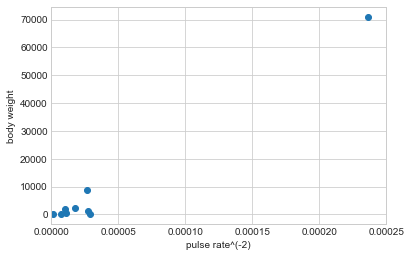
\includegraphics[width=0.5\linewidth]{s2_3/b.png}
		\end{figure}
		The proportionality constant is about $3\times 10^8$. So, the model is
		\[
		w = \frac{3\times 10^8}{p^2}
		\]
		where $w$ is body weight and $p$ is pulse rate.
	\end{enumerate}
\end{enumerate}
\end{document}

